\documentclass{article}

\usepackage{arxiv}
\usepackage[utf8]{inputenc} 
\usepackage[T1]{fontenc}    
\usepackage{hyperref}      
\usepackage{url}            
\usepackage{booktabs}       
\usepackage{amsfonts}       
\usepackage{nicefrac}       
\usepackage{microtype}      
\usepackage{cleveref}       
\usepackage{graphicx}
\usepackage{natbib}
\usepackage{doi}
\usepackage[portuguese]{babel}
\usepackage{caption}
\usepackage{braket}
\usepackage{amsmath}
\usepackage{algpseudocode}
\usepackage{algorithm}
\usepackage{mathtools}

\DeclarePairedDelimiter\floor{\lfloor}{\rfloor}

\newcommand{\tens}[1]{%
	\mathbin{\mathop{\otimes}\limits_{#1}}%
}

\setcounter{secnumdepth}{5}
\setcounter{tocdepth}{5}

\makeatletter
\renewcommand\subsubsubsection{\@startsection{paragraph}{4}{\z@}{-2.5ex\@plus -1ex \@minus -.25ex}{1.25ex \@plus .25ex}{\normalfont\normalsize\bfseries}}
\newcommand\subsubsubsubsection{\@startsection{subparagraph}{5}{\z@}{-2.5ex\@plus -1ex \@minus -.25ex}{1.25ex \@plus .25ex}{\normalfont\normalsize\bfseries}}
\makeatother


\title{Quantum Oracles - Como transformar problemas clássicos em quânticos}

\date{}


\author{ \href{https://orcid.org/0009-0008-9134-5974}{
\includegraphics[scale=0.06]{orcid.pdf}\hspace{1mm}Alexandre Silva}\\
	Ciências da Computação\\
	UNIVEM - Centro Universitário Eurípides de Marília\\
}

\graphicspath{ {../images/} }


\renewcommand{\headeright}{}
\renewcommand{\undertitle}{}
\renewcommand{\shorttitle}{}


\hypersetup{
	pdftitle={Quantum Oracles - Como transformar problemas classicos em quanticos},
	pdfsubject={quantum computing, computer science, ciencias da computacao, computacao quantica, algoritmos, algorithms},
	pdfauthor={Alexandre Silva},
	pdfkeywords={quantum oracles, quantum, quantum computing, algoritmos, algorithms},
}

\begin{document}
\maketitle
\begin{abstract}
	A partir do uso de quantum Oracles e outros fatores quânticos, como a superposição, foram feitos \emph{5 mini-projetos}. O objetivo desses projetos foi tentar responder se é possível transformar certos problemas em quânticos e se realmente tal transformação vale a pena. Após os testes foi possível ver que, há casos em que a versão quântica apresenta um aproveitamento igual ou um pouco superior em alguns casos, contudo ainda é necessário o uso de computadores clássicos para conseguir melhores resultados.
\end{abstract}


\section{Introdução}
Hoje, não é difícil ver alguém falando sobre computação quântica e como essas máquinas vão mudar o nosso futuro. Contudo, muitas dessas frases acabam se levando por extrapolações e/ou usos indevidos de ficção. Neste artigo, mostrarei que nem tudo é possível ser feito com um computador quântico atual, assim como existem pequenas áreas que se beneficiam ao máximo dessa nova tecnologia.\\
Para esse feito, serão mostrados \emph{5 mini-projetos} usando o \href{https://www.ibm.com/quantum/qiskit}{qiskit}, \emph{framework open source} da \href{https://www.ibm.com/}{IBM} para computação quântica, e resultados obtidos após executar os algoritmos quânticos e seus relativos em computação clássica.\\
Tais mini-projetos foram os seguintes: Explorador de Arquivos \ref{file-explorer}, conversão de milhas para quilômetros \ref{conversion}, Torres de Hanoi \ref{hanoi}, Buckshot Roulette \ref{buckshot} e QRAM \ref{qram}. Todas as implementações podem ser encontradas nesse  \href{https://github.com/Dpbm/scientific-initiation-1-quantum-oracles}{repositório do GitHub}.
Para a criação desses algoritmos, foram usados os Quantum Oracles explorando alguns efeitos quânticos para cada caso específico. 

\section{Oracles}
Partindo da ideia das \emph{Oracle Turing Machines} \cite{SOARE2009368}\cite{amreen_oracle}\cite{kalyanasyndaram_2021_mod04lec23}\cite{e21080800}, os Oracles são modelos matemáticos ideais, usados para abstrair certas partes de um algoritmo principal, em formato de caixa preta, facilitando a análise do algoritmo, assim como sua descrição matemática. Tais máquinas podem ser vistas também como uma função, recebendo entradas $x$ e retornando $f(x)$ em tempo $O(1)$. Em computação clássica, esse modelo não possui implementação real, sendo usado apenas descrições formais para problemas de decisão.\\
Contudo, em computação quântica, é possível implementar esses componentes e tomar proveito de sua estrutura e efeitos quânticos para conseguir um \emph{Speed-up} em relação aos algoritmos clássicos, como mostrado pelo algoritmo de Deutsch–Jozsa \cite{Fan_2007}. Além disso, os Oracles possuem um papel importante ao demonstrar a complexidade de um circuito, alguns dos meios utilizados são: profundidade (\emph{depth}), calculando o maior caminho que uma informação percorre no circuito, ou ainda a quantidade de gates aplicados. No entanto, essas maneiras acabam se prejudicando ao \emph{transpilar} o circuito para uma outra máquina, variando então a complexidade de acordo com a topologia e com os gates fisicamente implementados. Para solucionar isso, outra maneira de calcular é inserir partes do circuito em um Oracle, e descrever sua complexidade a partir da quantidade de vezes que ele chamado, também conhecido como \emph{query complexity} \cite{odonnell_2015_lecture} \cite{e21080800}.

\subsection{Tipos de Oracles}

A partir da definição dos Quantum Oracles, podemos classificá-los em relação a suas estruturas e maneiras de computar os dados.

\subsubsection{Phase Oracle}

O Phase Oracle, é o formato mais conhecido e usado em circuitos quânticos. Algoritmos como os de  Deutsch–Jozsa, Grover, Simon e Bernstein–Vazirani, tomam proveito desse artificio para se sobressair em relação às soluções clássicas. 

\subsubsubsection{Funcionamento Padrão}

Seu funcionamento, se baseia em atribuir uma fase global ao circuito, tomando proveito de fatores como \emph{Phase Kickback} (fase passa do target do CNOT e é aplicado no qubit de controle), para  conseguir modificar valores em superposição.

\begin{center}
	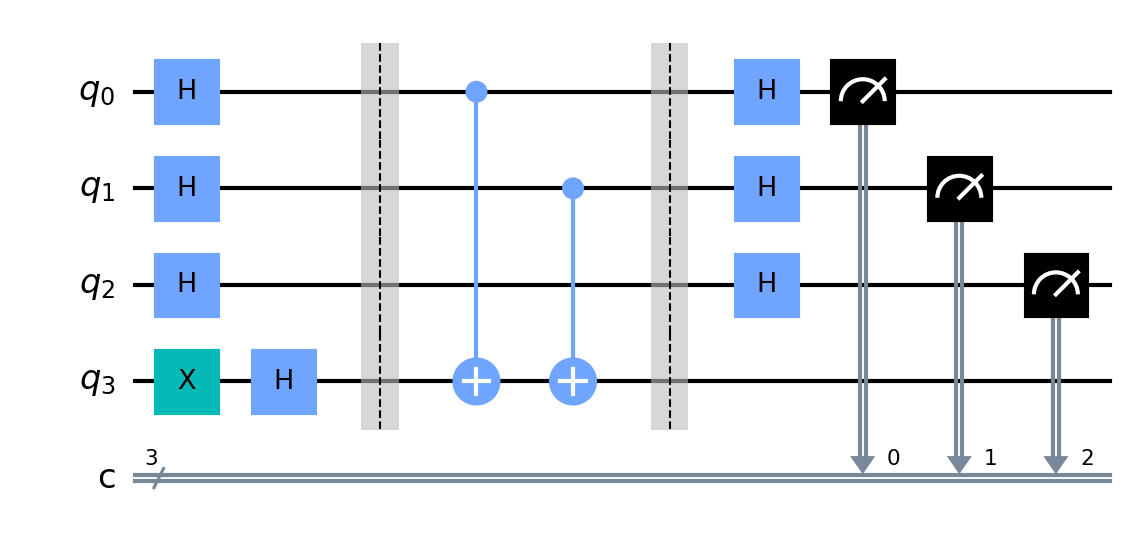
\includegraphics[scale=0.3]{phase_oracle_1.png}
	\captionof{figure}{Exemplo - Phase Oracle}
	\label{fig:phase-oracle-1}
\end{center}

Na Imagem \ref{fig:phase-oracle-1}, foi introduzida uma fase $\pi$ no qubit auxiliar ($q3$) através do estado  $\ket{-}$. Essa fase será responsável pode modificar os valores na matriz unitária do circuito. Nessa configuração, os CNOTs agem de uma forma um tanto diferente do convencional, aqui,  ao invés de apenas inverter o valor do qubit no target quando o qubit no control for $1$, devido a fase, ele também agirá como um gate $Z$ no control. Sendo assim, ao aplicar $CNOT\ket{-}\ket{+}$ (qubit menos significativo à direita), o estado se torna ${\frac{1}{\sqrt{2}}}{(\ket{0}\ket{-} - \ket{1}\ket{-})}$, e ao remover a superposição com o $H$, a saída se torna: ${\frac{1}{\sqrt{2}}}{(\ket{+}\ket{1} - \ket{-}\ket{1})}$. Dessa forma, o qubit que antes estava como controle do gate, sofre a ação do \emph{Phase Kickback}, e seu estado padrão $\ket{0}$ é modificado pela fase e se torna $\ket{1}$. A partir disso, é possível encodar um certo valor binário dentro do Oracle e utilizá-lo para cálculos. 

\subsubsubsection{Versão Minimal Oracle}

Além disso, esse não é o único formato possível de Phase Oracle. Por apenas aplicar uma fase em certas bit-strings, o qubit auxiliar pode ser removido e a fase pode ser adicionada através de gates $Z$controlados (ou outro gate capaz de aplicar uma fase $\pi$ para certa bit-string), mas ainda assim mantendo a natureza unitária, podendo ser visto também como um Minimal Oracle.
\\
\begin{center}
	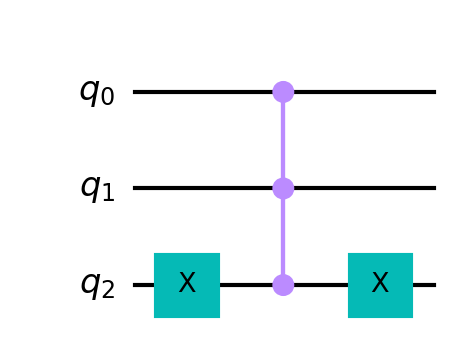
\includegraphics[scale=0.3]{phase_oracle_2.png}
	\captionof{figure}{Exemplo Phase Oracle como um Minimal Oracle}
	\label{fig:phase-oracle-2}
\end{center}


No exemplo da imagem \ref{fig:phase-oracle-2}, foi adicionado um gate $MCP$ com a fase global $\pi$ e dois gates $X$ para inverter quais qubits queremos que tenham o valor $0$, codificando assim o valor $011_{2}$ ou $3_{10}$.

\begin{center}
	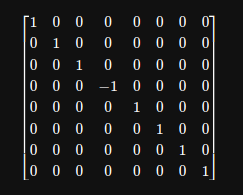
\includegraphics[scale=0.5]{phase_oracle_unitary.png}
	\captionof{figure}{Matriz unitária do Phase Oracle da imagem \ref{fig:phase-oracle-2}}
	\label{fig:phase-oracle-unitary}
\end{center}

É possível verificar então que ao criar esse circuito, é mantida a matriz identidade mas com a fase ($-1$) no valor $1$ na coluna relativa à $011_{2}$. 


\subsubsection{Boolean Oracle}

O Boolean Oracle, por sua vez, apresenta um funcionamento semelhante ao do Phase Oracle. Contudo, neste não é provida uma fase. Dessa forma, o Oracle age como uma função Booleana convencional, mapeando as entradas para valores de saída.

\begin{center}
	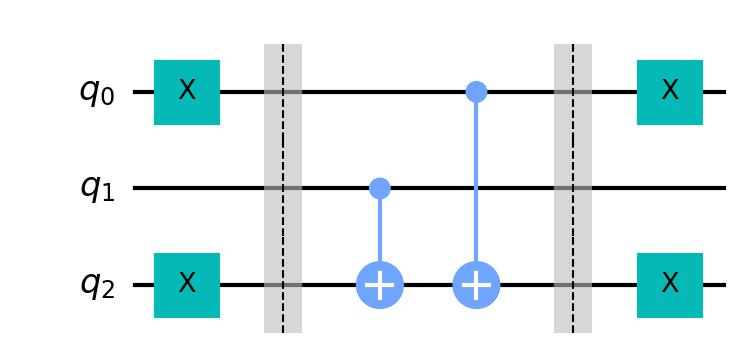
\includegraphics[scale=0.3]{balanced-oracle.png}
	\captionof{figure}{Exemplo de Oracle Booleano}
	\label{fig:boolean-oracle}
\end{center}

O Oracle implementado na figura \ref{fig:boolean-oracle}, pode ser reutilizado para o algoritmo de Deutsch-Jozsa. Basta apenas introduzir uma fase, e o Boolean Oracle se comportará como um Phase Oracle.

\subsubsection{Minimal Oracle}

Como já citado anteriormente, o Minimal Oracle possui uma função que, em sua essência, é unitária, não requerendo qubits adicionais. Sendo assim, este pode ser tanto Booleano como um Phase Oracle dependendo de sua implementação.

\begin{center}
	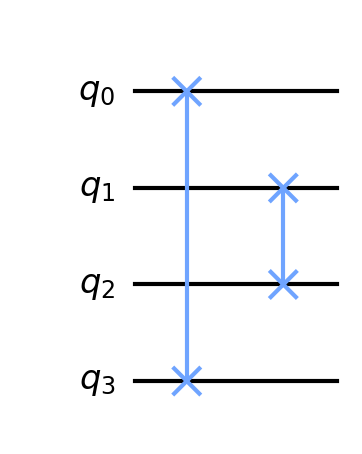
\includegraphics[scale=0.3]{minimal-oracle.png}
	\captionof{figure}{Exemplo de Minimal Oracle}
	\label{fig:minimal-oracle}
\end{center}

No exemplo da figura \ref{fig:minimal-oracle}, foram utilizados dois $SWAP$ para inverter a ordem dos valores. Com isso, a matriz final ainda se mantém unitária, com apenas valores invertidos em certas posições.


\subsubsection{QFT(Quantum Fourier Transform)}

O QFT, em suma, é um algoritmo quântico usado para projetar os valores da base computacional para a base $X$ (ou também conhecido como base de Fourier), ou vice-versa usando sua função inversa $QFT^{-1}$. Esse algoritmo, toma como base a transformada discreta de Fourier e aplica essa transformação em estados quânticos.\\
Mesmo sendo um algoritmo por si só, sua aplicação em circuitos se dá seguindo o formato de Oracles.

\begin{center}
	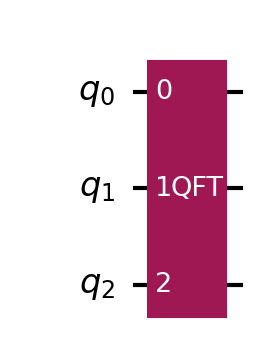
\includegraphics[scale=0.3]{QFT_1.png}
	\captionof{figure}{Exemplo do Oracle de QFT}
	\label{fig:QFT}
\end{center}

\begin{center}
	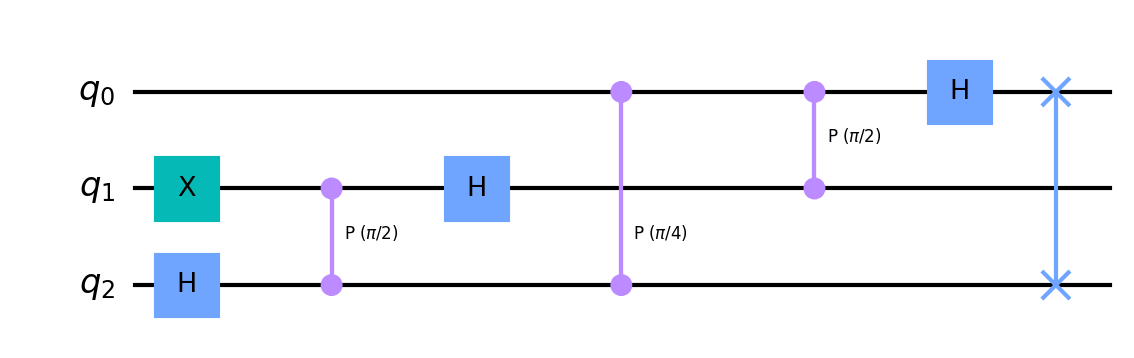
\includegraphics[scale=0.3]{QFT_1_transpiled.png}
	\captionof{figure}{Exemplo do Oracle de QFT transpilado usando o simulador AER do Qiskit}
	\label{fig:QFT-transpiled}
\end{center}

\begin{center}
	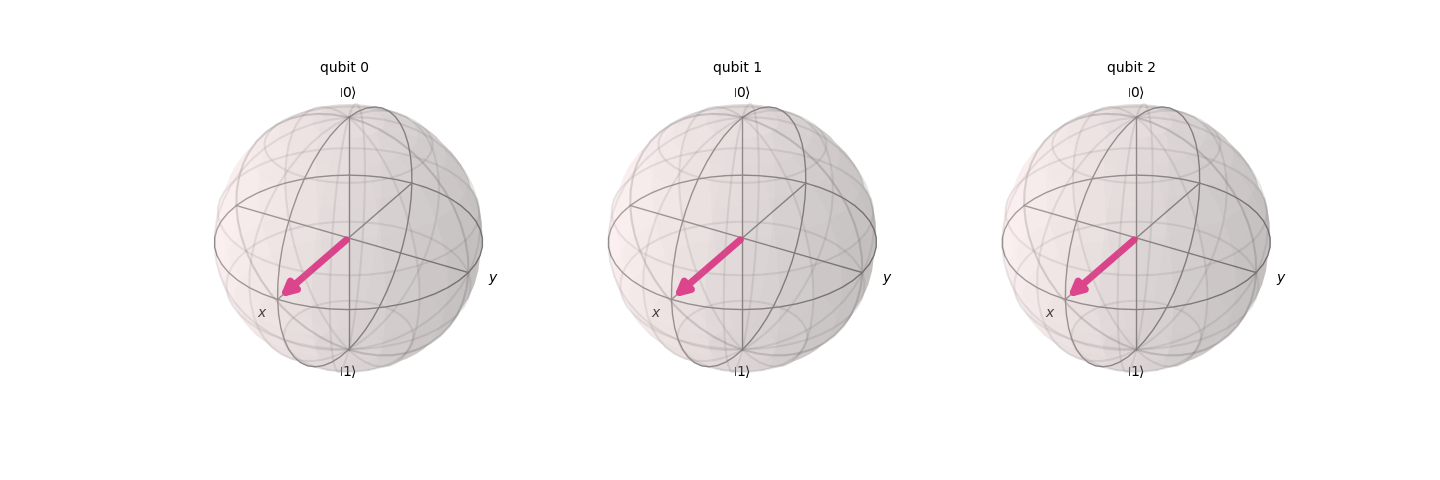
\includegraphics[scale=0.3]{QFT_1_bloch.png}
	\captionof{figure}{Valores mapeados na base de Fourier}
	\label{fig:QFT-bloch}
\end{center}


\subsubsection{Outros Oracles}

Além dos Oracles citados, é possível encontrar na literatura citações descrevendo o Oracle de Simon, o Oracle de Deutsch-Jozsa, etc. No entanto, esses são implementações de Oracles já citados e, além disso, para o desenvolvimento deste projeto, os Oracles mais relevantes são o Phase Oracle e o Boolean Oracle. Portanto, não há a necessidade de profundas investigações para essas subcategorias de Oracles.


\section{Desenvolvimento}

Com alguns algoritmos testados, e com o uso dos Oracles em mente, os 5 mini-projetos foram desenvolvidos da seguinte forma:

\subsection{Explorador de Arquivos} \label{file-explorer}

Imagine um computador quântico com um sistema operacional quântico (semelhante aos computadores convencionais, mas dessa vez seguindo as leis da mecânica quântica). Pensando nas partes desse sistema operacional, como seria possível pegar arquivos da memória usando a computação quântica?


\subsubsection{Algoritmos usados}

\subsubsection{Grover}
Um dos algoritmos mais comuns para a área é o algoritmo de Grover. Esse algoritmo realiza buscas em "bancos de dados"(bit strings) desorganizados em tempo $O(\sqrt{2^n})$ onde $n$ é o número de qubits usados. Nele, usamos um circuito do qual amplifica-se a probabilidade de encontrar os valores marcados no Oracle na saída.
Tal algoritmo segue o seguinte padrão: \
\begin{enumerate}
	\item{Configuramos todas as possíveis bit strings, ou seja aplicamos uma superposição uniforme $H^{\tens{^n}}$}
	\item{aplicamos o phase oracle $Uf$ do qual implementa uma função que marca os valores que desejamos encontrar}
	\item{aplicamos o operador de Grover Diffuser, $\mathbb{I} - 2 \ket{s}\bra{s}$}, sendo $s$ o estado com o valor que queremos
\end{enumerate}

Convertendo para um circuito temos algo semelhante a:


\begin{center}
	\includegraphics[scale=0.3]{Grover.png}
	\captionof{figure}{Exemplo algoritmo de Grover}
	\label{fig:grover-default-circuit}
\end{center}

Para 1 ou 2 valores, podemos usar a configuração acima. Mas maiores quantidade de valores, precisamos adcionar o conjunto Oracle + Diffuser $k$ vezes, sendo $k \approx { {\pi \over {4 \sqrt{a\over{2^n}}}} - {1\over2}  }$, sendo $a$ o numero de valores marcados.

\subsubsection{Diferença de conjuntos}

Utilizando os phase oracles, podemos criar dois Oracles distintis com ranges de valores diferentes e sobrepor seus valores, realizando a operação de diferença de conjuntos.

\begin{center}
	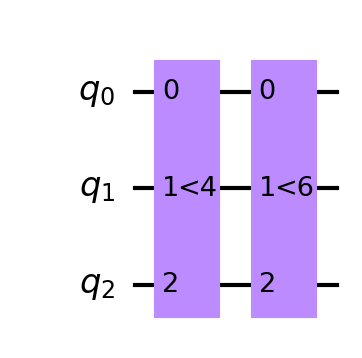
\includegraphics[scale=0.3]{less_than.png}
	\captionof{figure}{Exemplo de diferença de conjuntos}
	\label{fig:less-than-circuit}
\end{center}

Nesse exemplo foi encodado no primeiro oracle o set $\{000, 001, 010, 0110\}$ e no segundo $\{000, 001, 010, 011, 100, 101\}$.

\begin{center}
	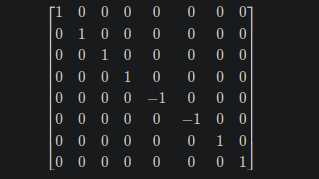
\includegraphics[scale=0.5]{less_than_unitary.png}
	\captionof{figure}{Resultado da diferença de conjuntos}
	\label{fig:less-than-circuit-unitary}
\end{center}

Como pode ser visto, apenas os valores $\{100, 101\}$ permaneceram com a fase, representando então a sobreposição delas.


\subsubsection{Solução para o problema}

Para a solução do problema, podemos criar em uma hash function $C(v)$ da qual recebe o path de um arquivo e retorna uma bit string respectiva. Com essa função em mãos, podemos utilizar o conjunto dos valores retornados e encoda-los em um phase oracle, agindo como uma especie de Look Up Table para os arquivos existentes na máquina.

No entando, para ter sucesso na pesquisa, é necessário utilizar um segundo Oracle encondando $S = P-s$, sendo $s$ o conjunto de arquivos do qual estamos procurando e $S$ os arquivos restantes, aproveitando-se então da diferença de conjuntos para encontrar então apenas os valores desejados para a pesquisa.


\begin{center}
	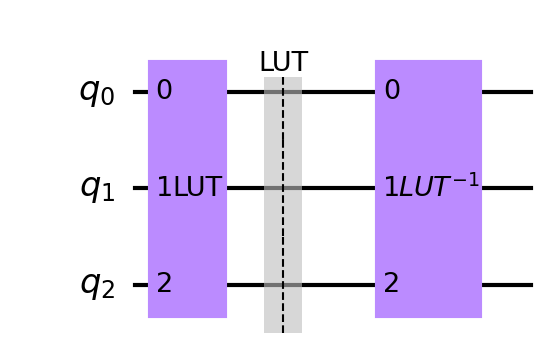
\includegraphics[scale=0.6]{sets-difference-look-up-table-oracle.png}
	\captionof{figure}{Diferença de conjuntos com as Look Up Tables}
	\label{fig:luts}
\end{center}

Sendo assim, o primeiro oracle age como o HD da marquina, marcando todos os arquivos existentes, e o segundo age como o mediador da pesquisa.

Com isso, adicionamos a Look Up Table final ao algoritmo de Grover.

\begin{center}
	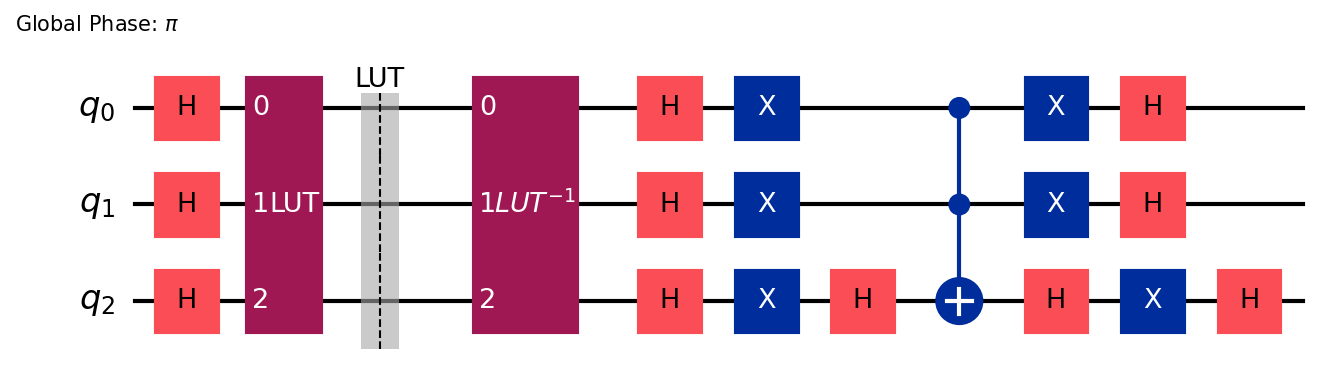
\includegraphics[scale=0.5]{file_explorer.png}
	\captionof{figure}{File explorer circuito}
	\label{fig:file-explorer}
\end{center}

\subsubsection{Resultados}

Para um caso hipotetico de sistema completamente quântico, certamente esse é um das maneiras de encontrar arquivos em meio a todos os outros.

Contudo, como o objetivo dessa pesquisa sugere, para utilizar esse modelo em um sistema clássico tomando proveito da computação quântica, não se mostra como a melhor opção.

Para sistemas convencionais, dos quais utilizam métodos baseados em árvores, não é possivel tirar qualquer proveito aqui, sendo $O$ polinomial contra $O$ quadrático.

Mesmo perante os testes clássicos feitos durante o desenvolvimento, esse protocolo só se mantém util quando a pesquisa era feita de forma linear.


\begin{center}
	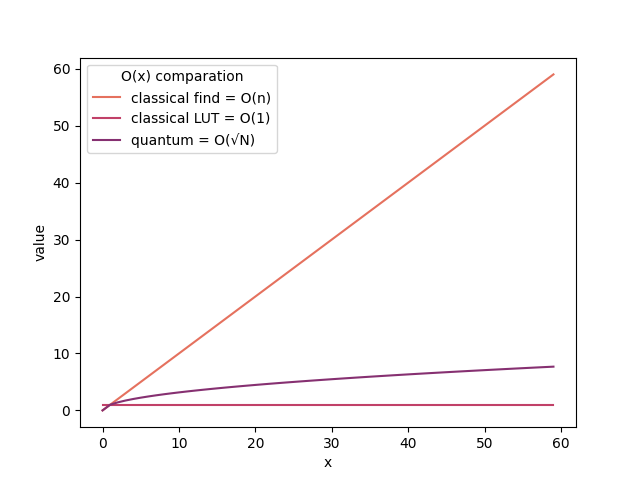
\includegraphics[scale=0.5]{algorithms-finding-comparation.png}
	\captionof{figure}{Comparação algoritmos usados na pesquisa}
	\label{fig:file-explorer-comparation-O}
\end{center}

Sendo assim, o algoritmo de Grover deve ser pensando para casos do qual a versão clássica possui complexidade $\ge O(n)$.


\subsection{Milhas para Quilômetros} \label{conversion}

O segundo problema testado foi a conversão de milhas para quilômetros. Essa ideia se deu após a descoberta de um algoritmo capaz de calcular a sequência de Fibonacci usando circuitos quânticos.

\subsubsection{Algoritmo Quântico de Fibonacci}

A versão quântica usada para calcular Fibonacci foi apresentada em \cite{gilliam2020canonical} e  demonstra que, utilizando um circuito que coloca em superposição todas as bit-strings com $n$ qubits, e então realizando operações para remover valores que possuem $1$s consecutivos, é possível encontrar o valor $n$ na sequência.

Esse circuito pode ser criado da seguinte maneira, como descrito no artigo original \cite{gilliam2020canonical}:

\begin{center}
	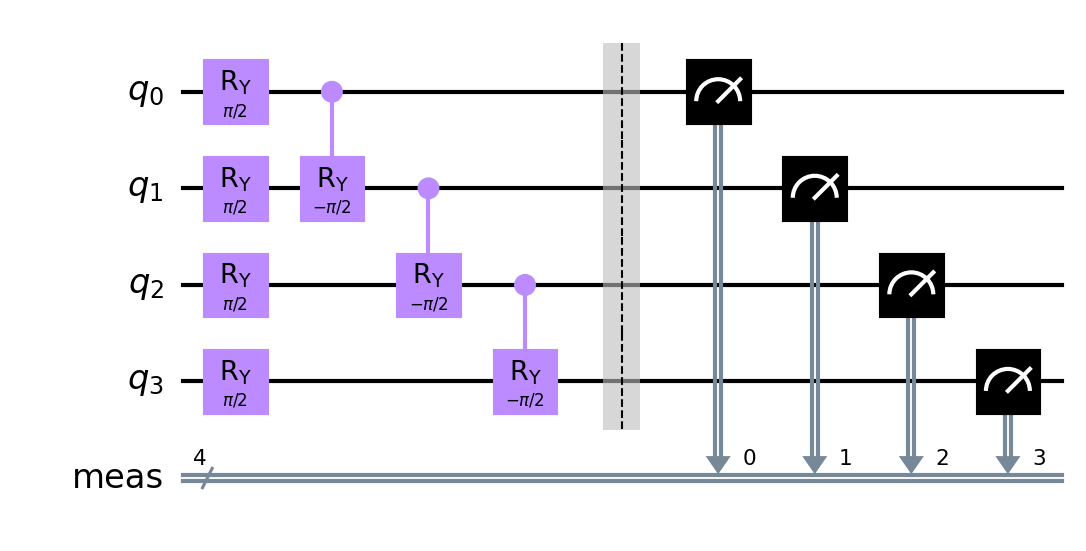
\includegraphics[scale=0.3]{fibonacci-circuit.png}
	\captionof{figure}{Exemplo Algoritmo Quântico de Fibonacci}
	\label{fig:fibonacci-circuit}
\end{center}

Assim, ao executá-lo, temos:

\begin{center}
	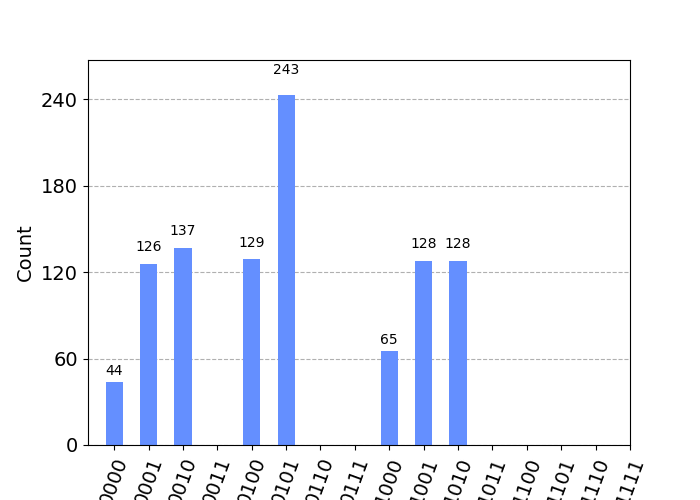
\includegraphics[scale=0.5]{fibonacci-4.png}
	\captionof{figure}{Resultado exemplo Fibonacci - F(4)}
	\label{fig:fibonacci-circuit-result}
\end{center}

Aqui, as bit-strings em si não são importantes para o resultado, mas apenas a quantidade de bit-strings diferentes que aparecem com valores não $0$s.\\ 
No exemplo em \ref{fig:fibonacci-circuit-result}, foram usados $4$ qubits para calcular $F(4)$. Assim, ao contar as bit-strings, temos $F(4) = 8$, retornando então o quarto valor da sequência (nesse caso, a sequência começa do valor $2$, seguindo dessa forma: $F(1)=2, F(2)=3, F(3)=5, F(4)=8, F(5)=13, F(6)=21, ...$). \\
Com isso, é possível usar esse circuito para computações de $F(n)$ utilizando $n$ qubits para encontrar o valor requisitado na posição $n$.

\subsubsection{Aproximação de Milhas para Quilômetros usando Fibonacci}

Para aproximar o valor de milhas para quilômetros, podemos utilizar a sequência de Fibonacci com a seguinte relação: $F_{km} = F_{milhas}(n+1)$, sendo aqui $F$ a versão clássica de Fibonacci com $F(1) = 1$ e $F(2) = 2$. Dessa forma, se a posição $n$ é conhecida, valor aproximado em quilômetros será dado em $n+1$.


\begin{table}[!h]
	\begin{center}
		\begin{tabular}{ |c|c| } 
			\hline
			milhas & km \\
			\hline
			1 & 2 \\
			\hline
			2 & 3 \\
			\hline
			3 & 5 \\
			\hline
			5 & 8 \\
			\hline
		\end{tabular}
	\caption{valores aproximados de Milhas para Quilômetros}
	\end{center}
\end{table}

Valores não presentes na sequência, podem ser aproximados repartindo o valor em partes menores lá presentes. Por exemplo, para transformar $10$ milhas em quilômetros, podemos fazer: $F(4+1) + F(2+1)$, ou seja $13 + 3 \approx 16$, aproximando então do valor mais preciso de $\approx 16.0934$


\subsubsection{Implementação do circuito}

Com essa formulação, foi criado um algoritmo clássico para quebrar um número desejado em partes menores, as quais podem ser calculadas em um circuito quântico, este então retorna tuplas mapeando a entrada para o valor $n_i$ e a quantas vezes que é necessário a sua aplicação $i$ sendo assim : $ f: (n) \to ((n_1, i), (n_2, i), ...)$.

O algoritmo final segue o fluxo:

\begin{algorithm}
	\begin{algorithmic}
		\State $partes \gets quebraValor(valorDeEntrada)$
		
		\For{parte in partes}
		
			Aplique o Oracle $F(parte)$
			
			Faça as medições nos qubits
			
			Reset os qubits usados
			
		\EndFor\\
		
		verifique o resultado de cada bit-string\\
		
		Multiplique cada resultado com o valor $i$ correspondente
		
	\end{algorithmic}
	\caption{Algoritmo quântico para a conversão}
	\label{alg:miles-to-km-quantum-algortihm}
\end{algorithm}

\begin{center}
	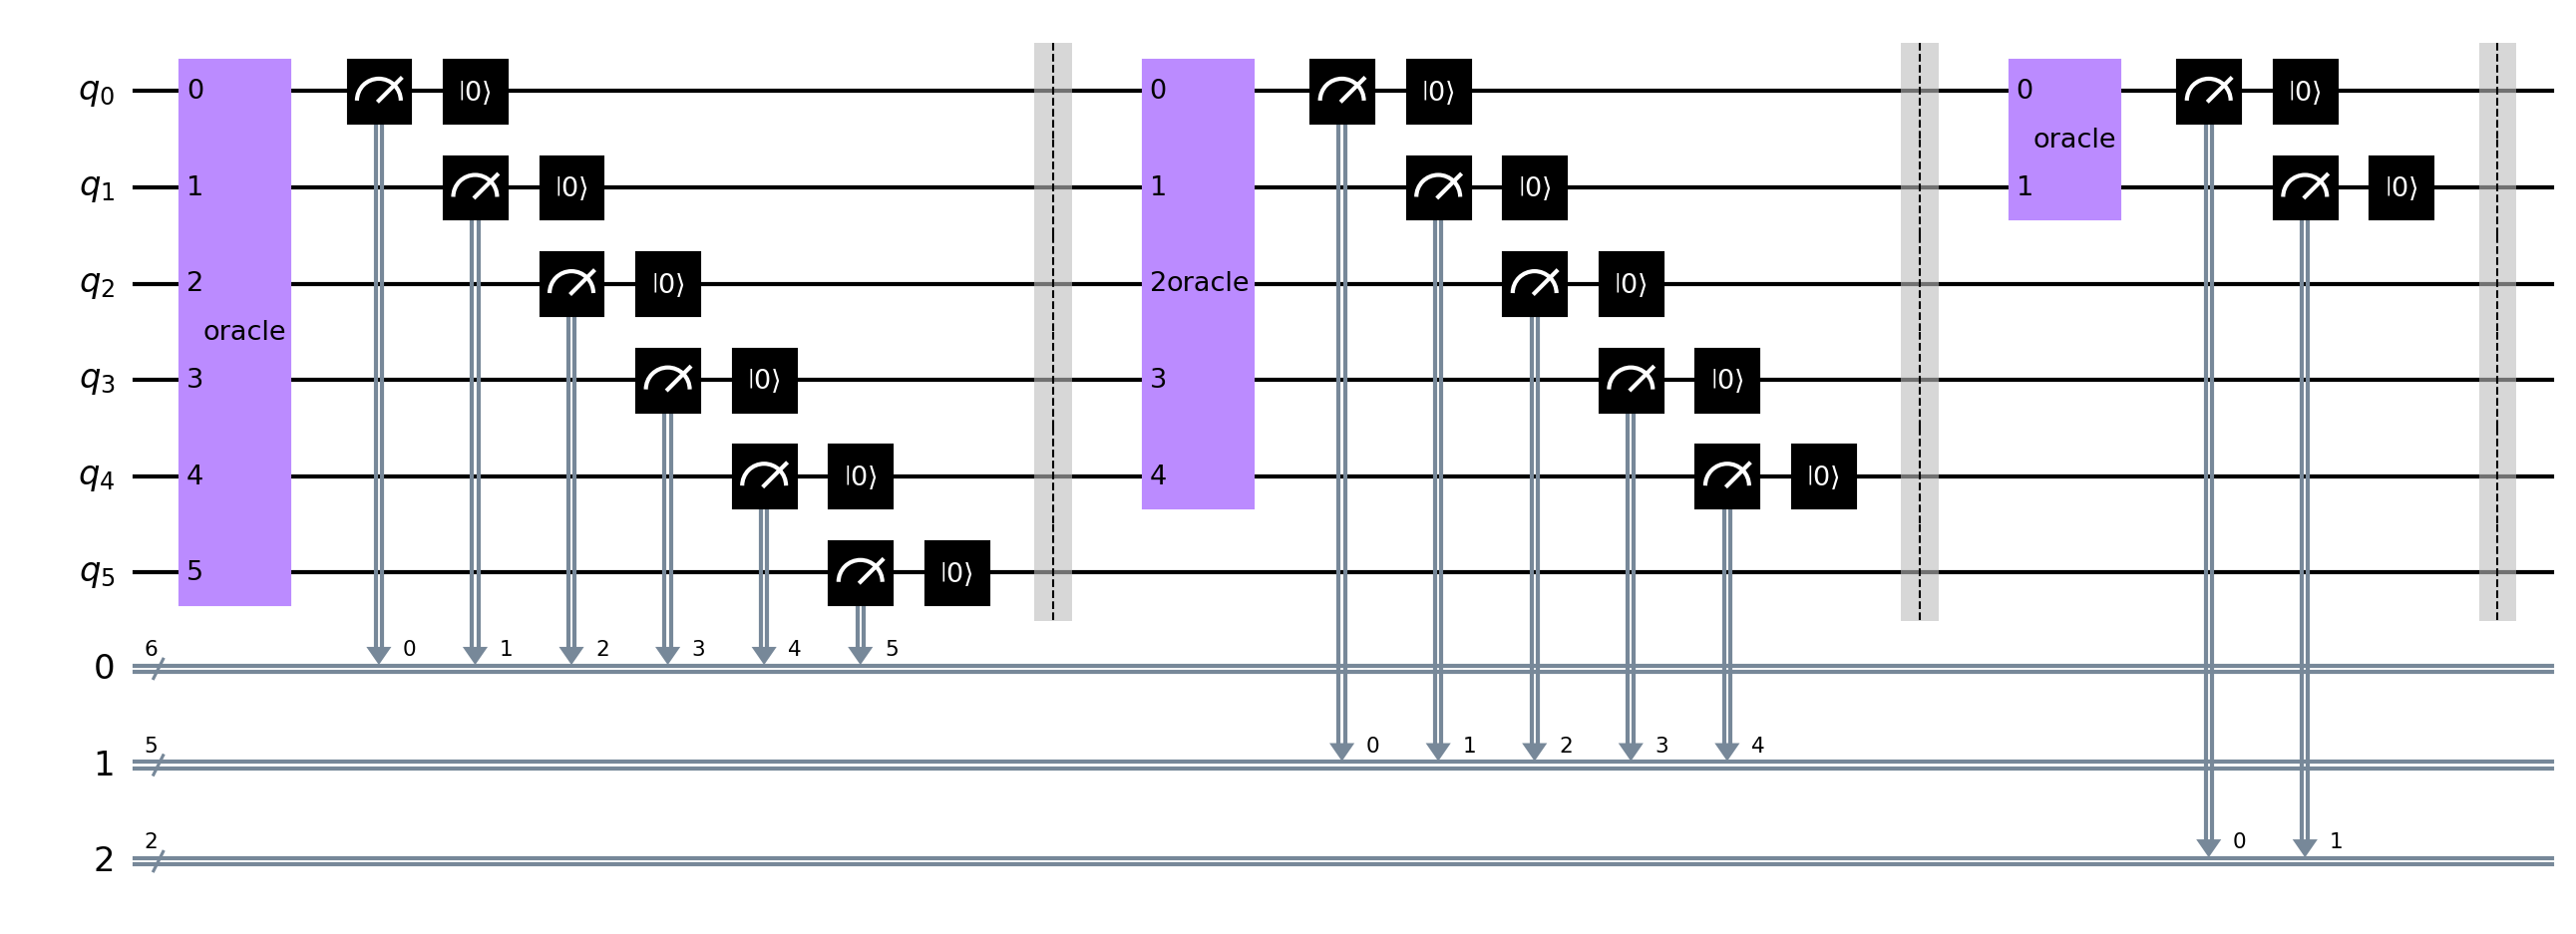
\includegraphics[scale=0.15]{number_breakdown_circuit.png}
	\captionof{figure}{Circuito de conversão}
	\label{fig:miles-km-circuit}
\end{center}

\subsubsection{Resultados}

Usando esse método é possível alcançar os valores esperados. Contudo existem alguns pontos que tornam esse método inviável:

\begin{enumerate}
\item{Quantidade necessária de medições e tempo de execução}\\
Para cada vez que medirmos o circuito, precisamos de uma quantidade alta de \emph{shots} para alcançar um resultado melhor, aumentando também o tempo necessário para executar.

\begin{center}
	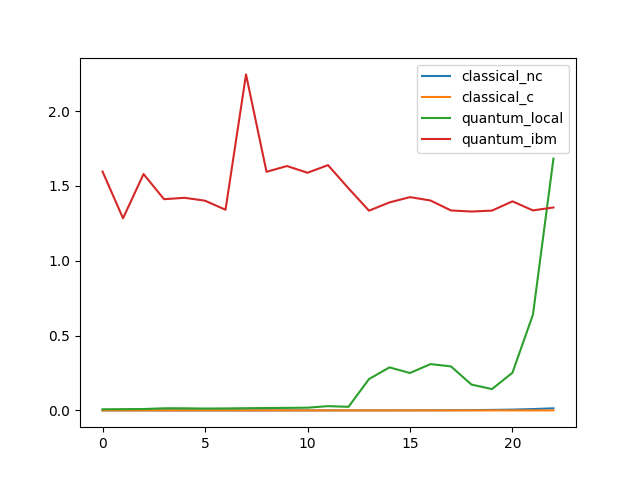
\includegraphics[scale=0.6]{comparison_miles_to_km.png}
	\captionof{figure}{Comparação tempos de execução}
	\label{fig:comparasion-miles-km-time}
\end{center}

Como mostrado em \ref{fig:comparasion-miles-km-time}, o tempo das versões clássicas, com e sem memoization, possuem tempos praticamente constantes em relação as versões quânticas.


\item{Erros}\\
Como a maioria dos algoritmos Quânticos da era NISQ(noisy intermediate-scale quantum), os erros também estão presentes, e por serem utilizados inúmeros gates multi-qubits, esses erros podem se intensificar de acordo com hardware usado.

\item{Imprecisão}\\

\begin{center}
	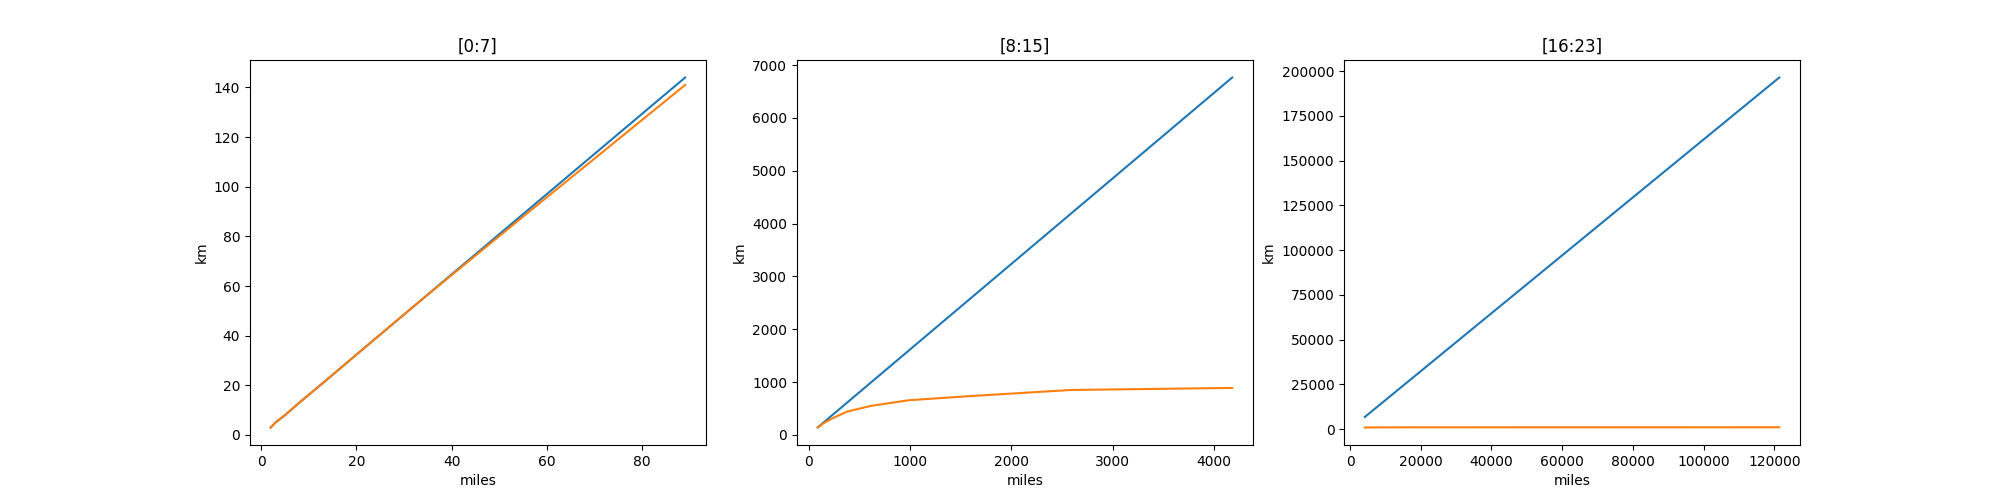
\includegraphics[scale=0.2]{miles_to_km_defiance.png}
	\captionof{figure}{Comparação resultados versão clássica e quântica}
	\label{fig:values-miles-km-quantum}
\end{center}

Como mostrado em \ref{fig:values-miles-km-quantum}, valores pequenos possuem uma boa precisão com os números esperados(em azul), mas a partir de certo ponto eles começam a se distanciar e perdem totalmente a precisão.

\item{Necessidade de intervenção clássica}

Por fim, esse algoritmo requer que primeiro seja verificado quais são os valores de Fibonacci necessários para cada parte(pré-processamento), além de ser necessário pós processamento após as medições. Sendo assim, a maior parte do tempo está sendo realizada computação clássica ao invés de quântica, o que acaba diminuindo a utilidade de um computador quântico aqui.

\end{enumerate}

Sendo assim, esse algoritmo não consegue se sair bem como a versão clássica, além de ser mais custoso na maioria dos casos. Para de fato evoluir essa implementação, será necessário remodelá-lo para um versão independente ou ainda com pouca computação clássica, priorizando a maneira como dados podem ser encodados e transformados no circuito.

\subsection{Torres de Hanoi} \label{hanoi}

Para a criação das torres de Hanoi, foi pensado em uma maneira de encodar a posição dos discos na torre utilizando seus valores binários e o Phase Oracle como meio de armazenamento.

\subsubsection{Implementação}

Para esse projeto, são necessários $(\floor{\log_2{x}} + 1) * 3$ qubits, sendo $x$ o número de discos. Estes seguem a ordem, $\ket{t_{n-1} t_{n-2} ... t_0}\ket{a_{n-1} a_{n-2} ... a_0}\ket{s_{n-1} s_{n-2} ... s_0}$, sendo $s$,$a$,$t$ a primeira, segunda e última torre respectivamente, e $n = {{n \space qubits} \over 3}$.

Com essa configuração, os números de $1$ à $x$ são codificados em seu formato binário nos qubits $s$, utilizando a fase global $\pi$. Em seguida, são realizadas operações de $swap$ bit-a-bit para mover os valores do $n$ $ls-$qubits  para os $n$ $ms-$qubits.

Para realizar essas operações, é necessário pré-calcular a sequência de movimentos usados  \cite{ldiaandr_2021_tower} \cite{diptokarmakar47_2019_how} \cite{a2020_towers}  \cite{geeksforgeeks_2014_program}. Dessa forma, essa versão quântica age como um jogador com uma lista de passos a serem seguidos, executando-os um-a-um.

\begin{center}
	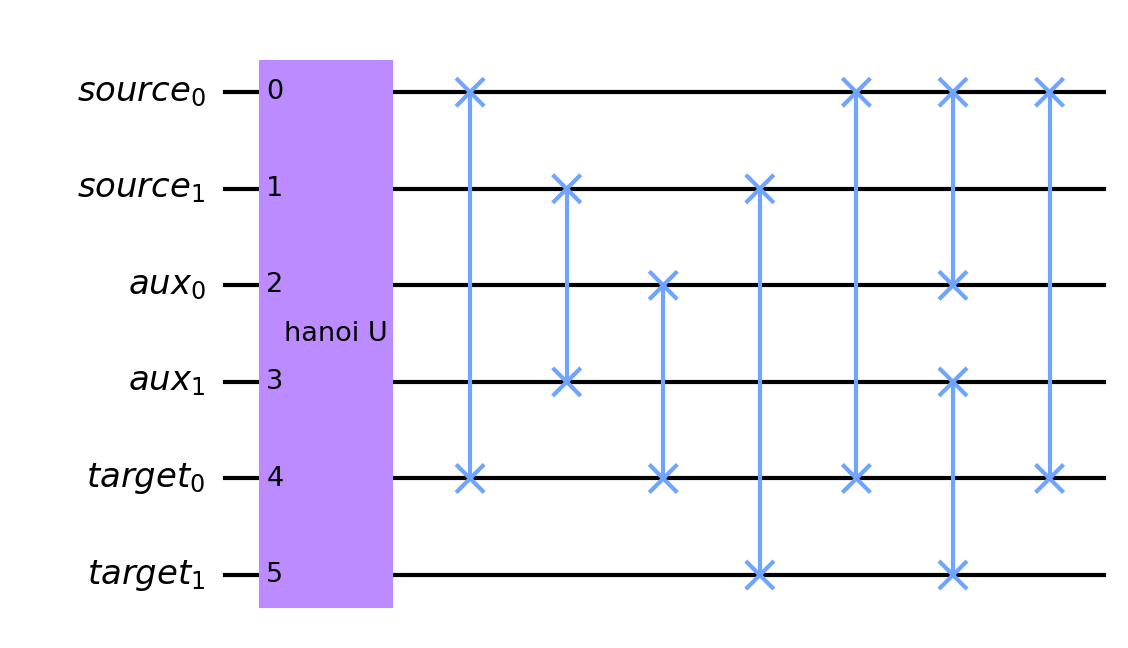
\includegraphics[scale=0.3]{hanoi_3_discs.png}
	\captionof{figure}{Torre de Hanoi com 3 discos}
	\label{fig:hanoi}
\end{center}

Nesse formato, pode-se utilizar outras partes no circuito, como o algoritmo de Grover, para verificar o resultado ou executar outras operações nos valores.

\begin{center}
	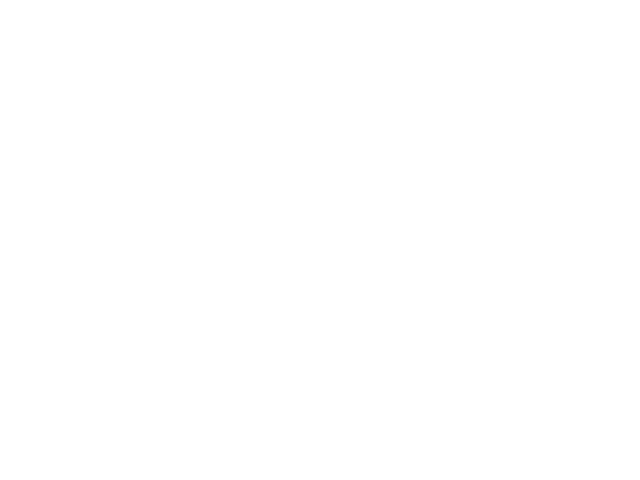
\includegraphics[scale=0.5]{result_hanoi_3_discs.png}
	\captionof{figure}{Resultado usando Grover - Torre de Hanoi com 3 discos}
	\label{fig:hanoi-result}
\end{center}

Em \ref{fig:hanoi-result}, os $3$ maiores resultados obtidos são as bit-strings com $01$, $10$ e $11$ nos bits mais significativos. Sendo assim, o resultado esperado para uma torre com 3 discos, foi atingido.

\subsubsection{Resultados}

Nessa versão, é seguida a mesma sequência do algoritmo clássico, necessitando, inclusive, de pré-processamento para conseguir a sequência de ações.\\
Em uma versão clássica, o movimento de retirar um disco de uma torre e move-lo para a próxima torre requer também esse pré-processamento, podendo ser realizado um-a-um ou tudo de uma vez antes da partida. Dessa forma, a versão clássica e quântica se igualam, não tendo ganhos ou perdas expressivas. 

\subsection{Buckshot Roulette} \label{buckshot}

Buckshot Roulette é um jogo feito pelo desenvolvedor \href{https://mikeklubnika.itch.io/}{Mike Klubnika} para computador que toma como base a premissa de reinventar a infame roleta russa. No jogo, você é desafiado por um demônio (dealer), e caso você ganhe você ganha uma recompensa, mas caso contrário o jogo reinicia.

Para esse projeto, tomamos como base a primeira rodada do jogo buscando encontrar a melhor estrategia para maximizar os ganhos.

Nessa primeira rodada temos 3 vidas, 2 balas falsas e 1 bala verdadeira.

A dinamica funciona da seguinte forma: você começa jogando,tendo duas possíveis escolhas, atirar em você mesmo ou no dealer. Caso você atire em você mesmo e a bala for real, você perde uma vida, mas você joga novamente na próxima rodada, caso a bala seja falsa você joga novamente. Agora, caso a escolha seja atirar no dealer, se a bala for real você ganha, se não o dealer joga.


\subsubsection{Versão clássica}

Antes de crair o circuito, foi feita a modelagem do jogo usando a estrutura em árvore.

\begin{center}
	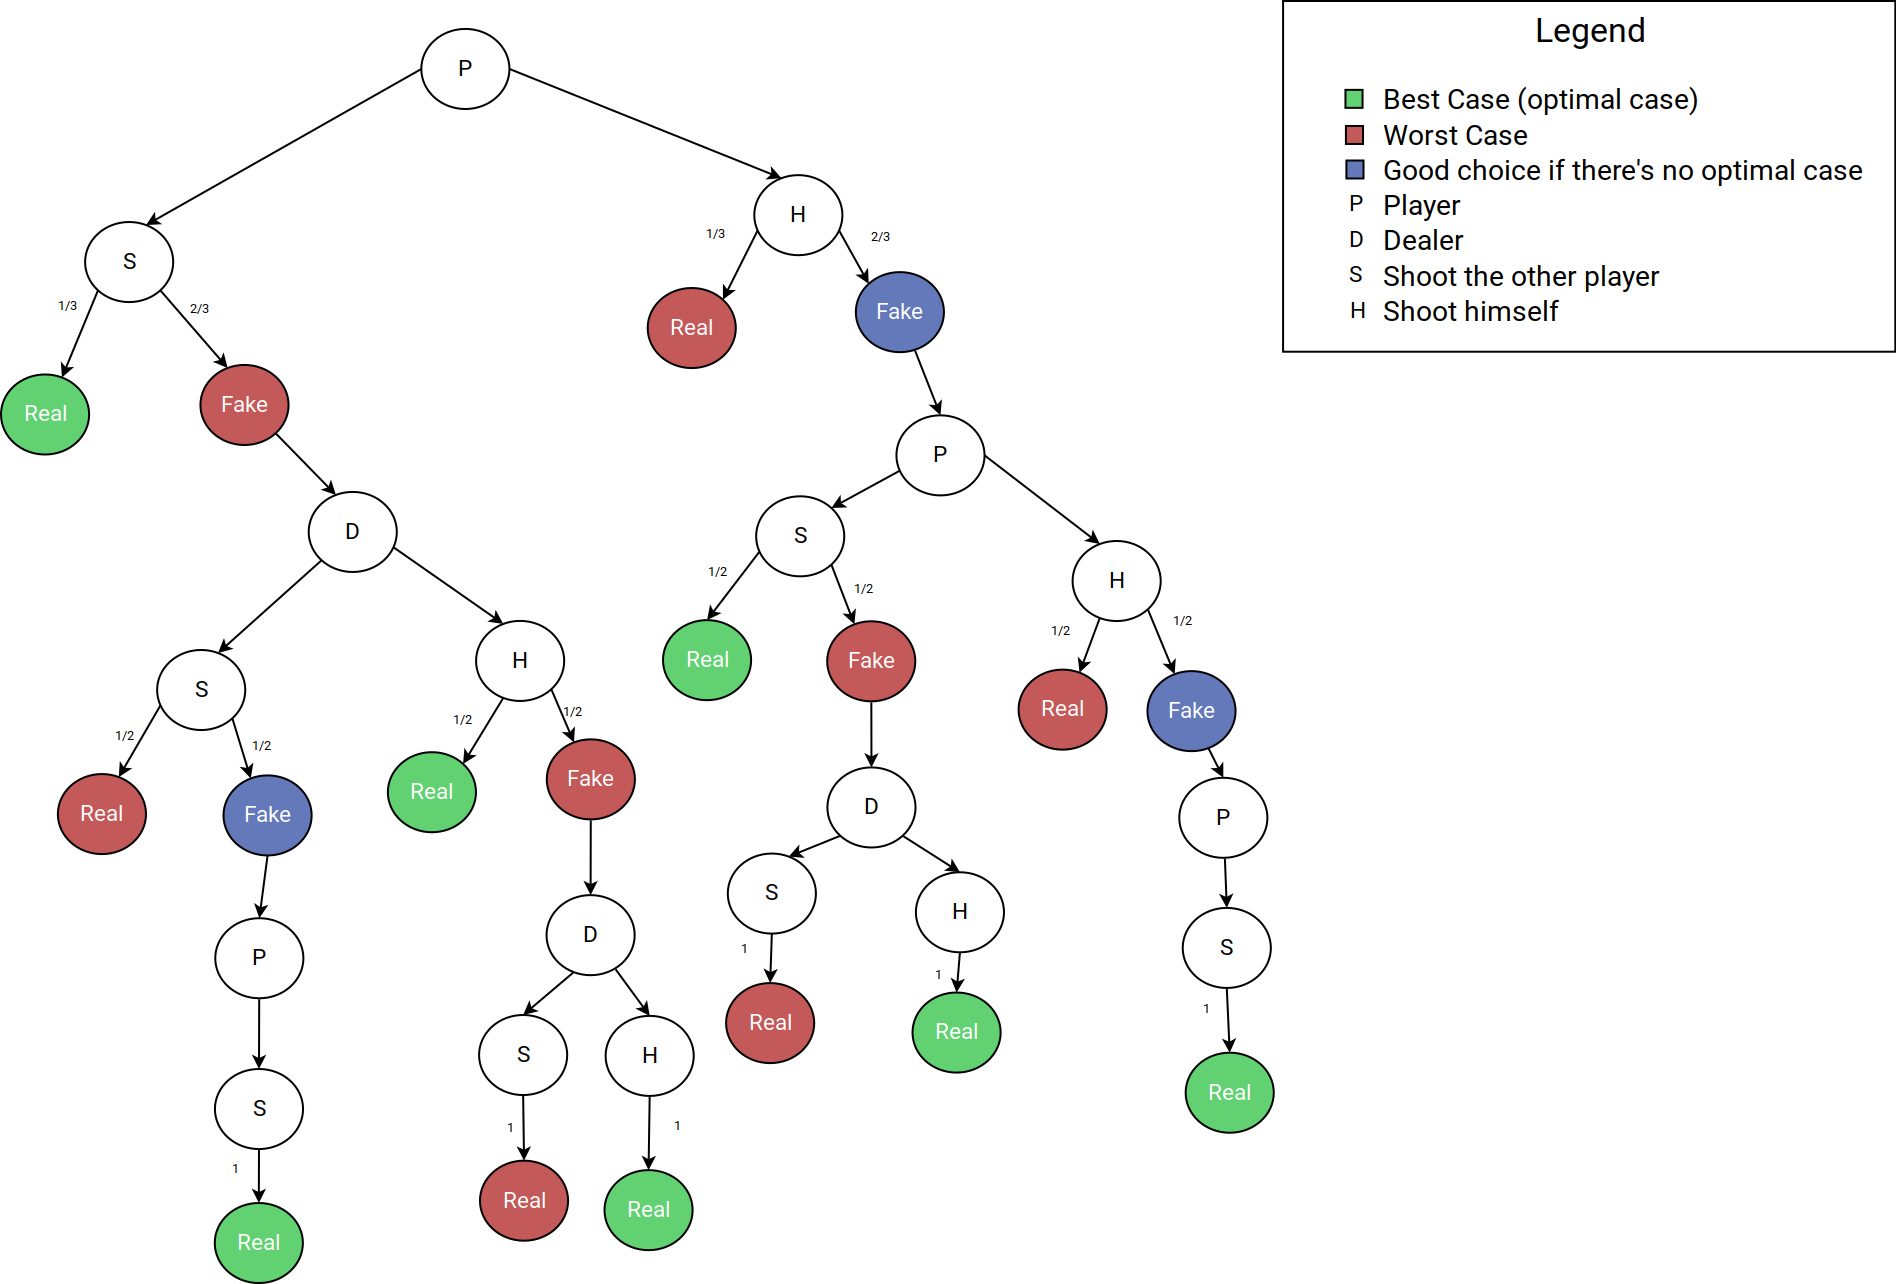
\includegraphics[scale=0.2]{buckshot-roulette-diagram.png}
	\captionof{figure}{Buckshot Roulette diagrama}
	\label{fig:classical-model-bckr}
\end{center}

Note que nessa estrutura, o dealer na ultima bala, ainda pode escolher atirar ou não nele mesmo, isso acontence pois o jogo implementa ações randomicas para o dealer.

Seguindo essa estrutura, podemos tentar encontrar o melhor caminho dentre a àrvore e simular os resultados da partida.


\begin{center}
	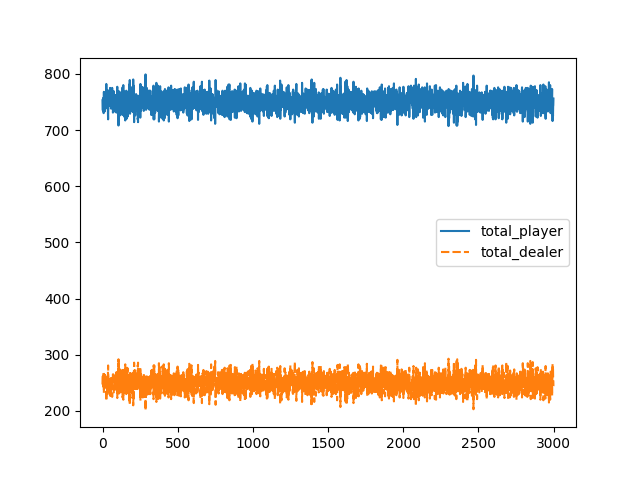
\includegraphics[scale=0.6]{optimal_player_strategy.png}
	\captionof{figure}{Buckshot Roulette clássico - melhor estratégia}
	\label{fig:classical-model-bckr-optimal-strategy}
\end{center}

Após testar os possíveis caminhso, o melhor resultado obtido foi esse apresentado acima em \ref{fig:classical-model-bckr-optimal-strategy}. Com um pouco de investigação, foi possível entender que a melhor estratégia encontrada foi o player começar atirando no dealer. Isso pois ao seguir tal caminho, ele tem uma chance a menos de perder a rodada, já que a chance de perder logo no começo é eliminada.




\begin{table}[!h]
	\begin{center}
		\begin{tabular}{ |c|c|c|c| } 
			\hline
			rodada & ação & resultado da ação & resultado da partida \\
			\hline
			1 & player atira no dealer  & real & player ganha\\
			\hline
			1 & player atira no dealer  & fake & -\\
			\hline
			2 & dealer atira no player  & real & dealer ganha\\
			\hline
			2 & dealer atira no player  & fake & -\\
			\hline
			2 & dealer atira nele mesmo  & real & player ganha\\
			\hline
			2 & dealer atira nele mesmo  & fake & -\\
			\hline
			3 & player atira no dealer  & real & player ganha\\
			\hline
			3 & dealer atira no player & real & dealer ganha\\
			\hline
			3 & dealer atira nele mesmo  & real & player ganha\\
			\hline
		\end{tabular}
		\caption{melhor estratégia - possíveis resultados}
	\end{center}
\end{table}

\subsubsection{Versão quântica}

A partir dessa ideia, um circuito quântico foi modelado imitando o primeiro round, e um oracle foi usado para cada jogador implementando sua estratégia em seu interior.

\begin{center}
	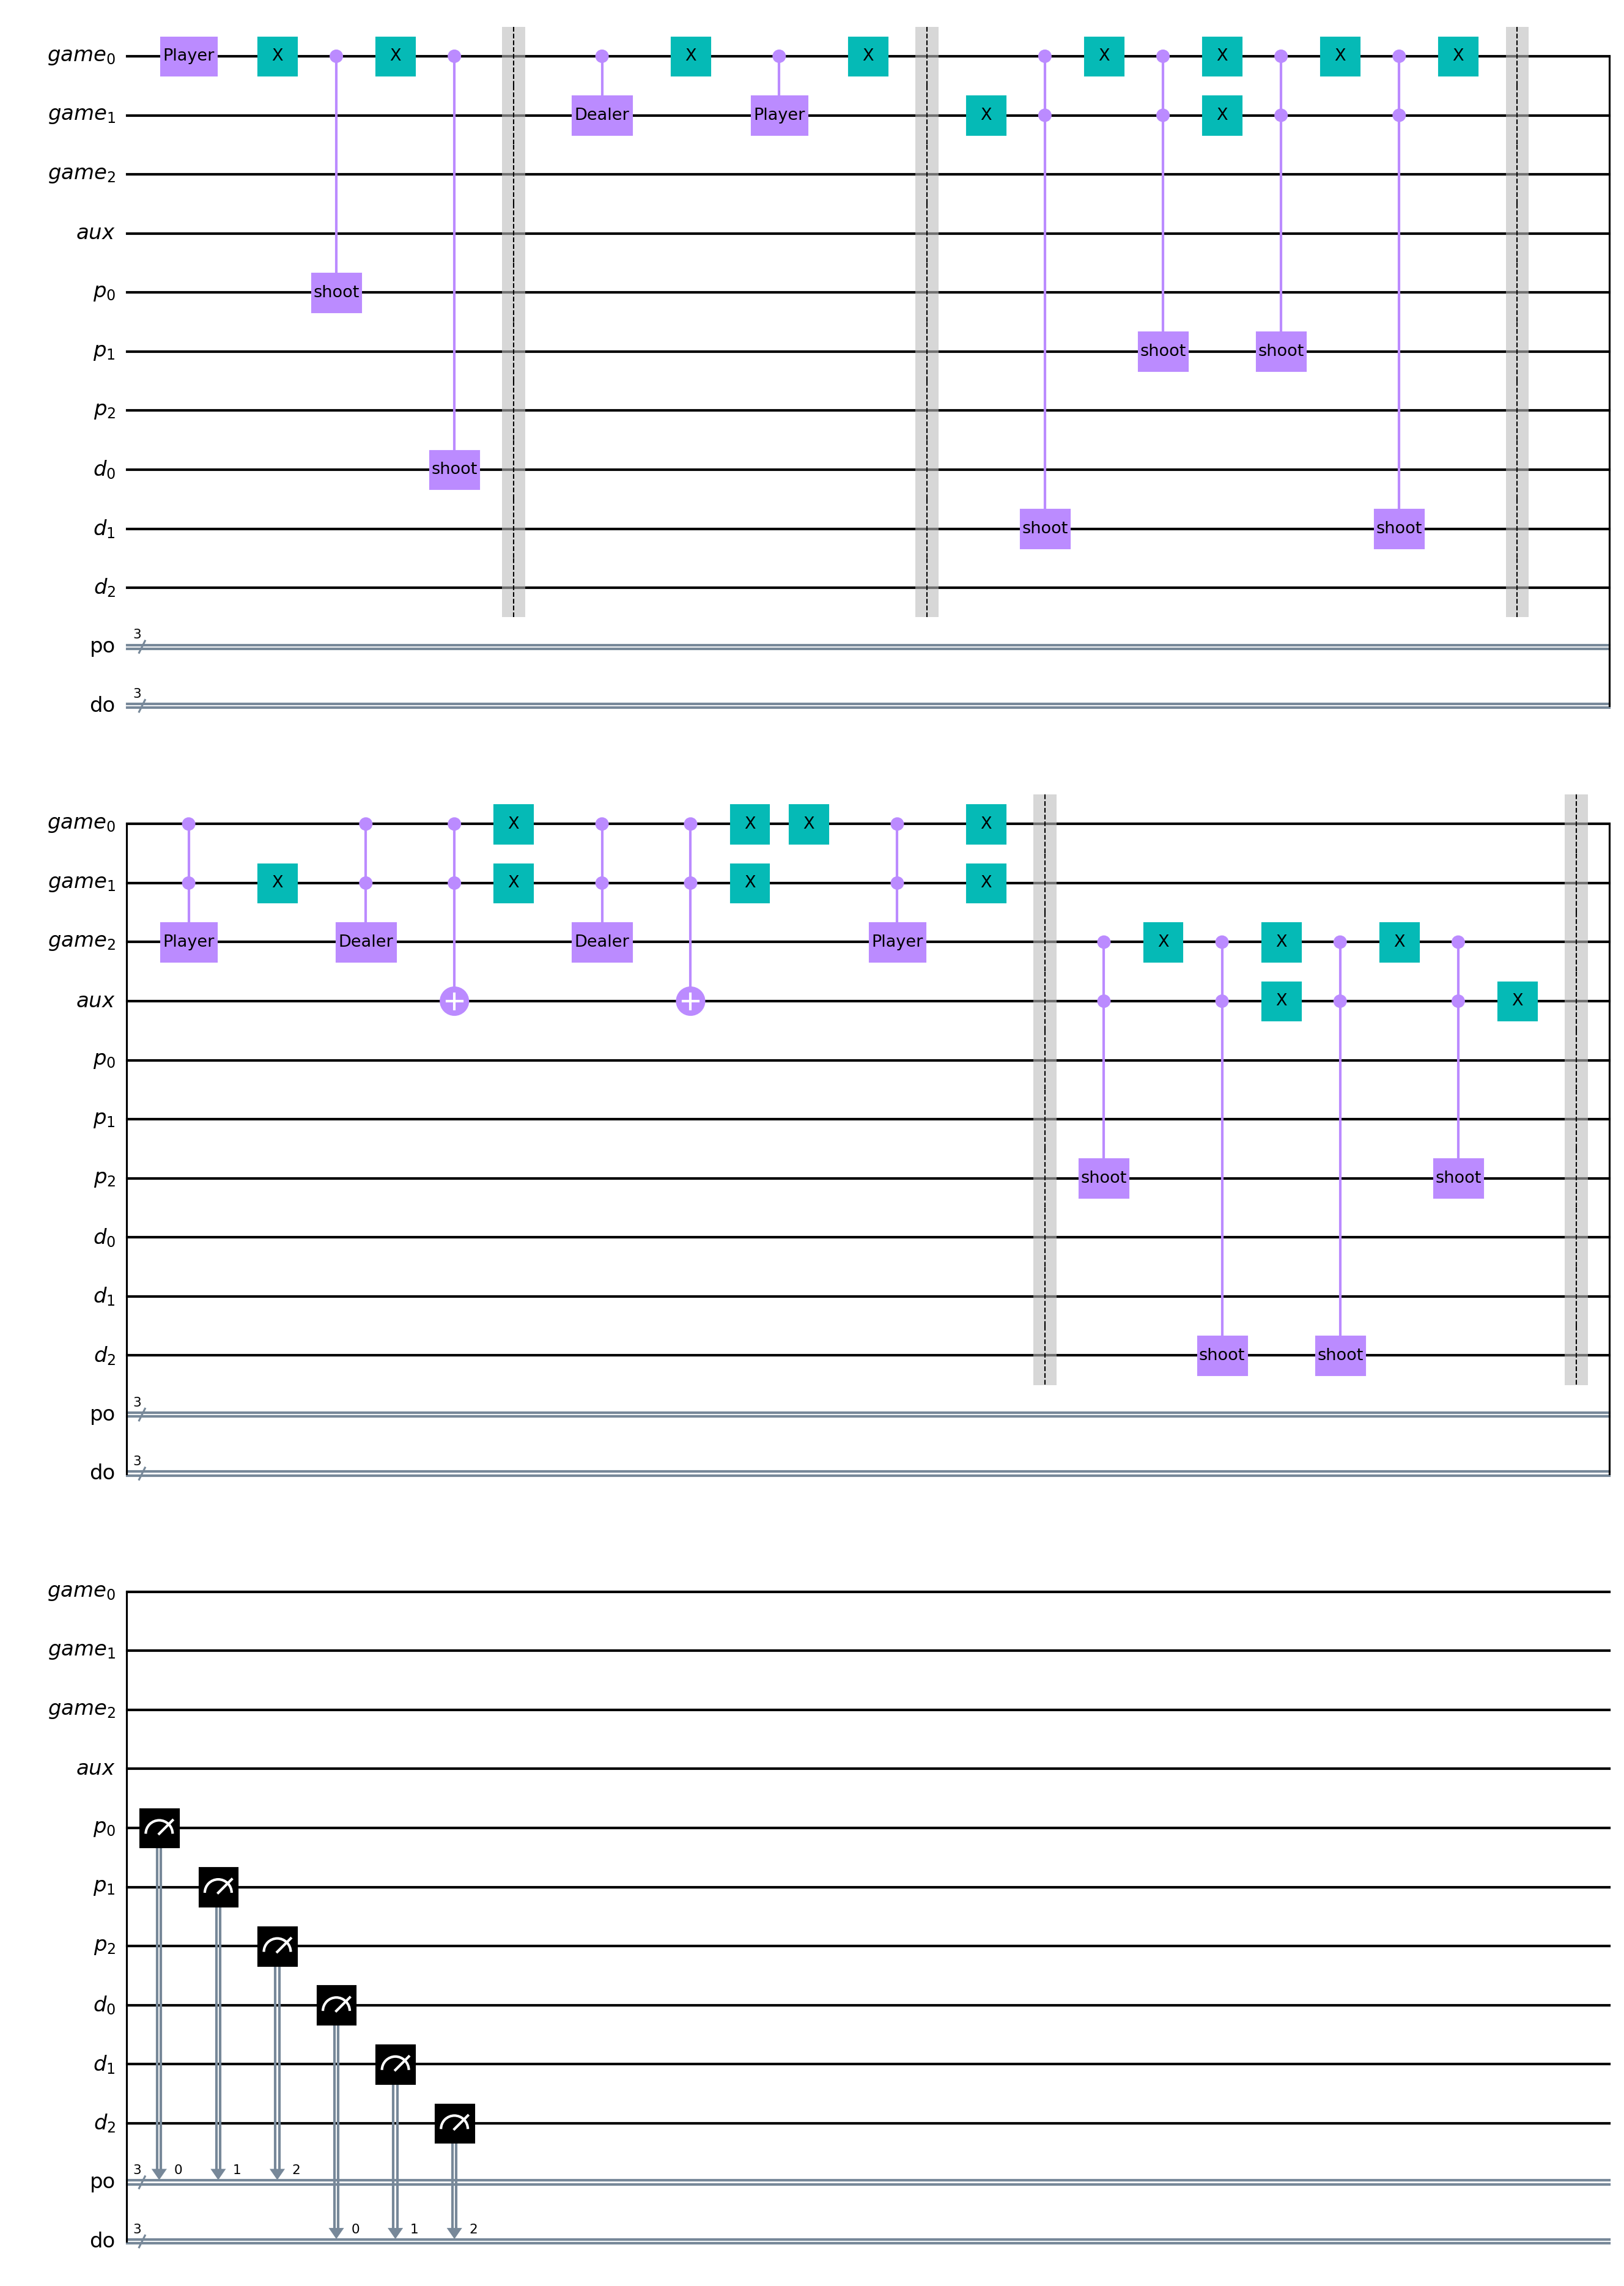
\includegraphics[scale=0.3]{quantum_buckshot_roulette.png}
	\captionof{figure}{Circuito para o buckshot roulette}
	\label{fig:bckr-circuit}
\end{center}

Além disso, para encontrarmos a melhor estratégia para o player, foi inserido dois parâmetros dentro do oracle, sendo possível inserir qualquer valor $\theta$ e $\phi$ para encontrar a melhor rotação na bloch sphere. 

Após verificar uma grande variedade de valores possíveis, a rotação que entregou o melhor resultado foi $\theta = 3.0853981633974477, \phi=5.685398163397447$.
Usando essa estratégia, os resultados foram semelhantes a versão clássica usando o simulador Aer:

\begin{center}
	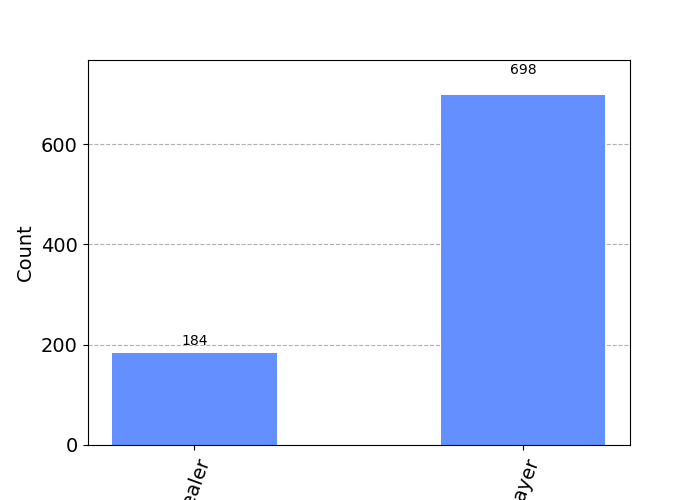
\includegraphics[scale=0.6]{final_buckshot_roulette_quantum_optimal_strategy.png}
	\captionof{figure}{Resultado Buckshot Roulette quântico}
	\label{fig:bckr-circuit-result}
\end{center}

Observando a bloch sphere do estado gerado por essa rotação, é possível ver também que a estratégia de fato se assemelha a versão classica, com o player preferindo atirar no dealer a maior parte do tempo (o valor 1 aqui representa atirar no outro jogador e 0 atirar em si mesmo).

\begin{center}
	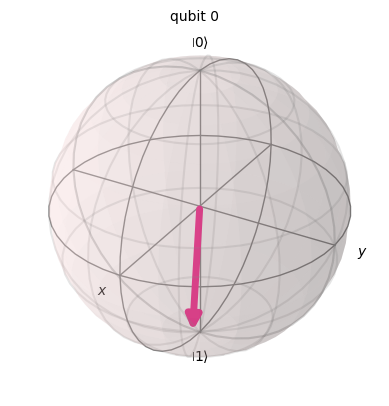
\includegraphics[scale=0.6]{player_optimal_strategy_bloch.png}
	\captionof{figure}{Melhor estratégia Buckshot Roulette quântico - Bloch Sphere}
	\label{fig:bckr-bloch-sphere-best-strategy}
\end{center}

\subsubsection{Conclusões}

Para esse problema, não há uma competição certa entre as duas versões, uma vez que uma é diretamente inspirada na outra.

Além disso, a versão quântica possui ainda a possibilidade de explorar mais valores do que a versão clássica, deixando o player mais aberto a escolha de estratégias.

Em relação a erros providos pelo hardware não afeta diretamente os resultados, uma vez que mesmo com os erros a proporção se mantém.


 \begin{center}
 	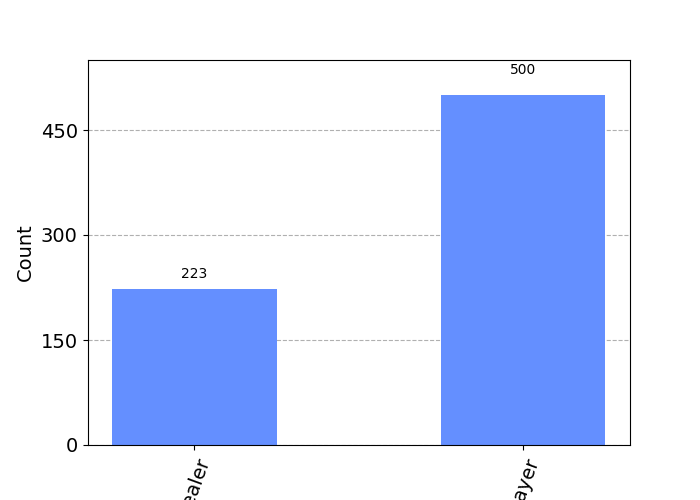
\includegraphics[scale=0.6]{final_buckshot_roulette_quantum_optimal_strategy_fake_melbourne.png}
 	\captionof{figure}{Resultados Buckshot Roulette usando o fake backend Melbourne da IBM}
 	\label{fig:bckr-fake-melbourne}
 \end{center}

Note também que o total de partidas ganhas não chega ao total jogado, 1000 partidas no total, isso pois, pelo design do circuito, não é possível verificar a jogada do player anterior, sendo possível continuar jogando mesmo que um dos players já tenham perdido, o que foi necessário correções usando pós processamento após a simulação.

Em suma, ambos as simulações atingiram o mesmo resultado e foi demonstrado que é possível usar aqui o quantum oracle como uma representação de um player dentro do circuito.

\subsection{QRAM} \label{qram}
Por fim, o último projeto realizado foi o de uma QRAM utilizando os oracles para encodar os valores desejados. Nessa versão, foi testado maneiras de criar QROMs (com dados estaticos dentro), e uma possível maneira de utilizar uma QRAM habil para escrita.

Neste, foi levado em consideração o armazenamento de estados quânticos, e não de bitstrings clássicas.

\subsubsection{QROM implementação}

Primeiro, foi feita uma versão de QROM, do qual utiliza $n$ qubits para endereços e $m$ qubits para a criação dos estados. Não necessáriamente os valores precisam estar correlacionados, podemos ter $n=3, m=10$. Isso pois, nesse formato, podemos mapear diversas superposições diferentes e aplicálas quando certo endereço for chamado. Sendo assim, o algoritmo aqui mostrado armazena os valores a partir da configuração de gates controlados interiores ao oracle, criando uma superposição apenas quando certo valor de entrada é inserido.

A entrada do circuito segue o seguinte formato: ${\ket{0}^{\tens^m}} {\ket{a_{n-1} a_{n-2} ... a_0}}$

\begin{center}
	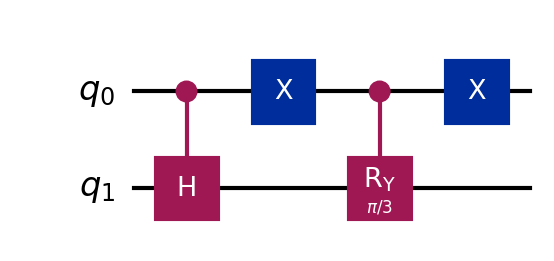
\includegraphics[scale=0.5]{qrom_1.png}
	\captionof{figure}{Exemplo circuito - QROM}
	\label{fig:qrom}
\end{center}

A partir desse circuito, podemos abristrair para um oracle e utilizar em um circuito maior, chamando-o novamente sempre que for necessário um certo estado ou ainda colocar os endereços em superposição e ter uma mistura de superposições na saída.

\begin{center}
	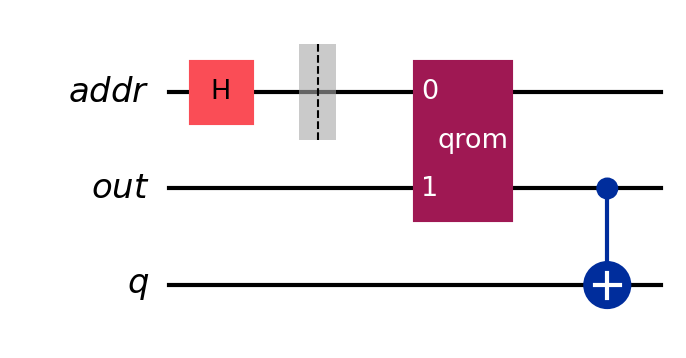
\includegraphics[scale=0.5]{qrom_1_usage.png}
	\captionof{figure}{Exemplo circuito usando a QROM}
	\label{fig:qrom-usage}
\end{center}

Nessa configuração, os estados em superposição serã colocados no qubit denominado \emph{out}, sendo possível se aproveitar dela em outros qubits, como nesse caso o qubit \emph{q}.

Contudo, devido ao no cloning theorem, não é possível copiar esse estado para outro qubit, então só é possível aqui se aproveitar dos qubits de saída, ou utilizada do teleporte de estados para destruir o estado interno do oracle e mover para outros qubits desejados.


\subsubsection{QRAM read and write - implementação}

Para criar uma QRAM com a possibilidade de escrever também, podemos exploarar o teleporte quântico já citado antes. Com isso, podemos ter $n$ qubits, sendo cada qubit um endereço único, e utilizar do teleporte para mover um estado que estava no circuito, para o dominio da QRAM.

 \begin{center}
 	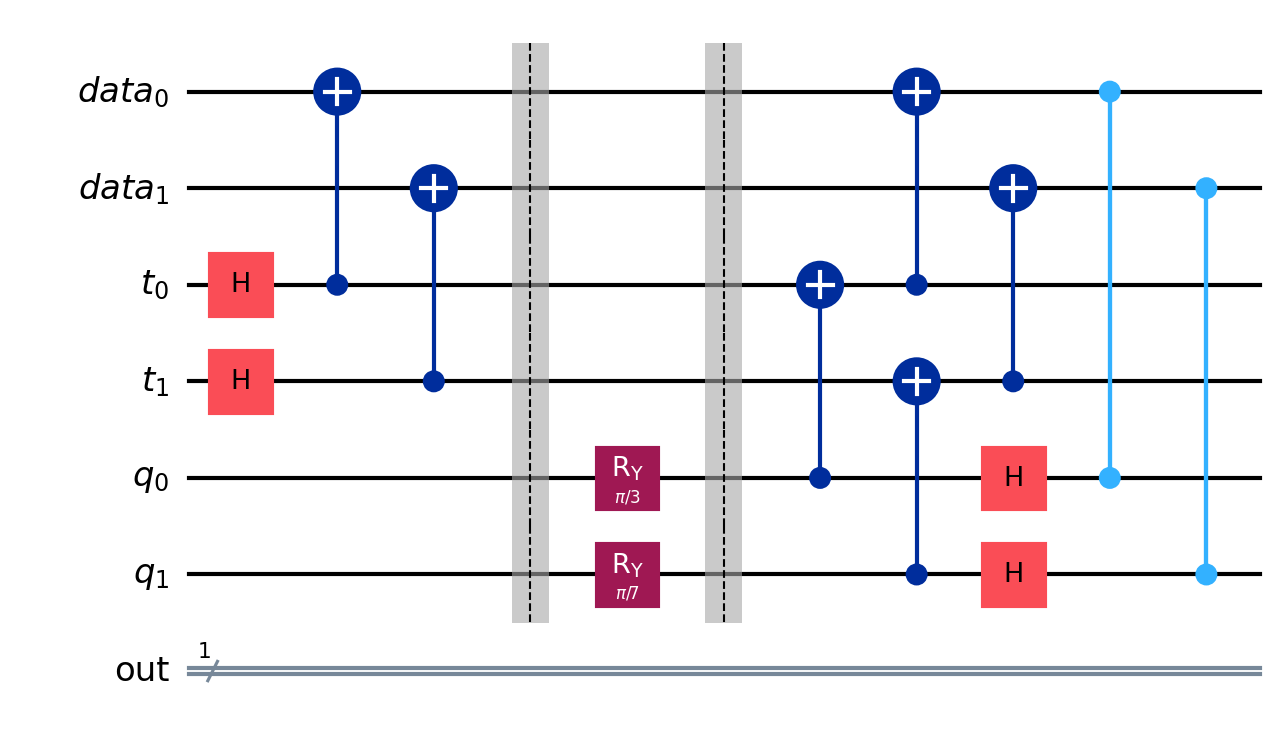
\includegraphics[scale=0.4]{qram.png}
 	\captionof{figure}{Exemplo circuito - QRAM}
 	\label{fig:qram}
 \end{center}

Aqui é necessário $n$ qubits para $n$ endereços (cada endereço aqui é um qubit de \emph{data}) e $n$ qubits para o teleporte (qubits nomeados como \emph{t}). Mesmo crescendo linearmente, podemos aqui utilizar sobreescrever valores nas posições desejadas, assim como interferir com outras superposições apenas teleportando novos valores para o qubit $i$.

\subsubsection{Conclusões}

Com esse projeto e com a literatura usada \cite{jaques2023qram}\cite{Giovannetti_2008}, é possível entender que versões quânticas de memória são dificeis de ser implementadas e ainda não foi possível tomar proveito do todo o seu pontecial usando as superposições e estados de outras bases a não ser a base computacional $({0,1})$.

Após as implementações, foi possível entender que, criar tais memórias pode parecer uma tarefa simples, mas devido a fatores como, complexidade de mapear dados, complexidade de utilizar a memória (já que é necessário reaplica-lá toda vez que for requisitado seu uso), no cloning, etc. Foi possível entender que tal modelo não é ainda viavel, sendo necessário mais pesquisadas focadas no tema, asim como possíveis implementações em um Hardware futuro.

Em suma, utilizar tais circuitos agora não é das tarefas mais faceis, assim como não necessariamente trará resultados no momento.


\subsection{Conclusão}

Com isso, foi mostrado que a computação quântica ainda tem muito potencial, contudo é possível ver que certos fatores prejudicam o seu uso no momento, assim como a falta de certos recursos.

No momento, é claro que computadores quânticos são máquinas extremamente úteis para diversos casos, e de fato existem áreas que tomaram extremo proveito com elas, como criptografia, machine learning, química, física, matemática, etc. Mostrando que a computação clássica não está condenada, mas sim uma nova era está surgindo com a junção da computação clássica e computação quântica.

Em resumo, é possível tirar proveito da computação quântica para problemas que conhecemos clássicamente. No entanto, é necessário averiguar se há algum fator quântico que pode explorar o problema de uma forma que classicamente seria impossível ou não usuais, como no caso dessa pesquisa os Oracles.




\nocite{SOARE2009368}
\nocite{odonnell_2015_lecture}
\nocite{bacon_2006_cse}
\nocite{lipics_stacs}
\nocite{odonnell_2015_lecture_2}
\nocite{brodkorb_2019_the}
\nocite{amreen_oracle}
\nocite{kalyanasyndaram_2021_mod04lec23}
\nocite{davis_2006_turing}
\nocite{viswanathan_2013_reductions}
\nocite{Fan_2007}
\nocite{cryptoeprint:2020/1270}
\nocite{buhrman1998quantum}
\nocite{sanchezrivero2023initial}
\nocite{gilliam2020canonical}
\nocite{Kashefi_2002}
\nocite{e21080800}
\nocite{Zeng_2014}
\nocite{atici2004comparative}
\nocite{sundarappan_2022_how}
\nocite{dai_view}
\nocite{sep-game-theory}
\nocite{Giovannetti_2008}
\nocite{jaques2023qram}
\nocite{PythonEWL2022}
\nocite{frackiewicz2011application}
\nocite{Eisert_1999}
\nocite{usman_2019_kilometres}
\nocite{ldiaandr_2021_tower}
\nocite{diptokarmakar47_2019_how}
\nocite{a2020_towers}
\nocite{geeksforgeeks_2014_program}
\nocite{khan_2021_quantum}
\nocite{legn_2022_dilemma}
\nocite{siegelwax_2022_quantum}
\nocite{landi_density}
\nocite{bacon_2006_cse}
\nocite{vijayakrishnan_2019_role}
\nocite{python_scientific}
\nocite{scipyoptimizeminimize_scalar}
\nocite{davis_optimization}
\nocite{scipyoptimizeminimize}



\bibliographystyle{unsrt}
\bibliography{references}


\end{document}
